\documentclass[PICOReport.tex]{subfiles}

\begin{document}

%% Beginning of Martin

The \ac{CMB} comes to us from the furthest reaches of the observable Universe, and its photons experience all of cosmic history.  Created when the Universe was a hotter, simpler place, CMB photons probe fundamental physics, provide exquisite measurements of the constituents of the cosmos, and test relativity.  On their journey they feel the impact of the gravitational potentials formed from the assembling cosmic web of superclusters, clusters, and galaxies.  They interact with the ionized gas in the inter- and circum-galactic medium, gas that eventually fuels star and galaxy formation.  Superposed upon the CMB is the emission from multiple extragalactic sources and from our Galaxy.  All of this leaves an imprint which sensitive measurements can disentangle so that CMB studies impact every aspect of cosmology and many areas of astrophysics.

\begin{wrapfigure}{R}{0.31\textwidth}  % r is right aligned, l is left. Capital letters allow figure to float on page.
\vspace{-5pt} % if move up and reduce to 12 lines only (add [12] before {R}) saves 1 line.
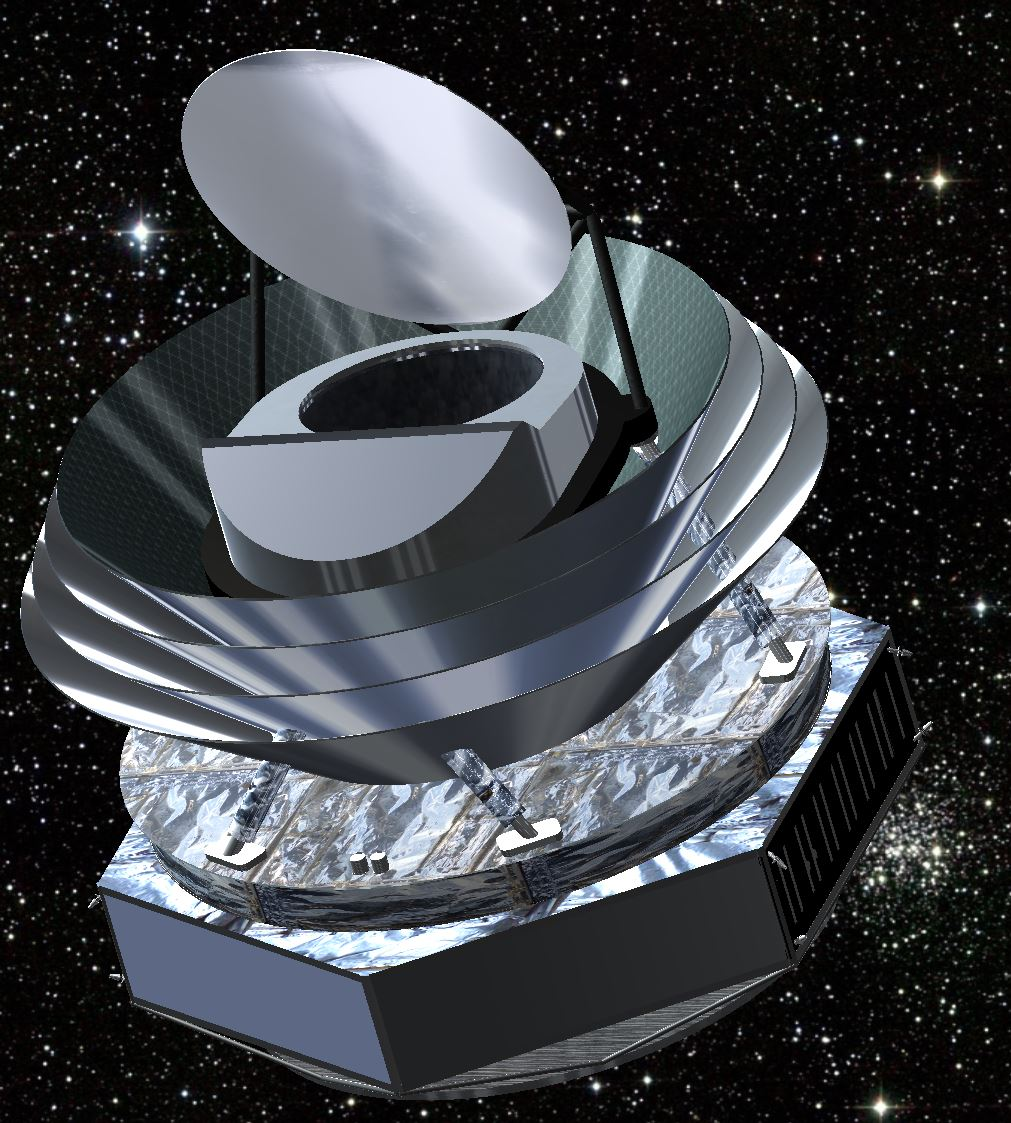
\includegraphics[width=0.31\textwidth]{images/PICO_Image.jpg}
\vspace{-0.25in}
\caption{\captiontext The PICO spacecraft 
\label{fig:pico_rendered} }
\end{wrapfigure}

Building upon a long legacy of successful measurements, the next decade holds tremendous potential for new, exciting \ac{CMB} discoveries.  Such discoveries, delivered by the Probe of Inflation and Cosmic Origins (PICO, Fig.~\ref{fig:pico_rendered}), promise to be revolutionary, affecting physics, astrophysics, and cosmology. PICO is an imaging polarimeter that will scan the sky for 5 years in 21 frequency bands spread between 21 and 799~GHz; see Tables~\ref{tab:specs} and \ref{tab:spec_bands}. It will produce ten independent full-sky surveys of intensity and polarization with a final combined-map noise level equivalent to 3300 \planck\ missions for the baseline required specifications, though in our current best-estimate it would perform as 6400 \planck\ missions.  
%It will produce the first ever full-sky polarization maps at frequencies above 350 GHz, and it will have diffraction limited resolution of 1' at 800~GHz. 

With these capabilities, unmatched by any other existing or proposed platform, PICO will have compelling and broad science deliverables. The mission will address the seven science objectives (SOs), which are listed in Table~\ref{tab:STM}. Delivering this set was the basis for selecting PICO's design and for setting instrument requirements. But PICO's science reach is broader than the baseline set. 

PICO could determine the energy scale of inflation and give a first, direct probe of quantum gravity (SO1, \S~\ref{sec:fundamentalsci}). The mission will attempt to detect the signal that arises from gravitational waves sourced by inflation and parameterized by the tensor-to-scalar ratio, $r$, at a level of $r =5\times10^{-4} \, (5\sigma)$. This level is 100 times lower than current upper limits, and more than 10 times lower than limits forecast by funded future experiments.  If the signal is not detected, PICO will constrain broad classes of inflationary models, exclude at $5 \sigma$ models for which the characteristic scale in the potential is the Planck scale, and distinguish between reheating scenarios at $3\sigma$ (SO1 and SO2). The combination of data from PICO and LSST could rule out all models of slow-roll single-field inflation, marking a watershed in studies of inflation. 
%If the signal is not detected, PICO will constrain broad classes of inflationary models and exclude at $5 \sigma$ models for which the characteristic scale in the potential is the Planck scale (SO1 and SO2). The combination of data from PICO and LSST can constrain features in the inflationary potential, the field content during inflation and could rule out all models of slow-roll single-field inflation, marking a watershed in studies of inflation. \comor{reword?}

The mission will have a deep impact on particle physics by measuring the expected sum of the neutrino masses with $4\sigma$ confidence, rising to $7\sigma$ if the sum is near 0.1~eV (SO3). Reaching the $4\sigma$ level can only be done with an instrument that can measure the polarization of the CMB on the largest angular scales, a measurement best done from space, which gives access to the full sky, and with a broad band of frequencies to remove foreground contaminants.  
Cluster counts provided by PICO in combination with followup redshift measurements, and PICO's map of the projected gravitational potentials along the line of sight in combination with the LSST gold sample of galaxies, will give two additional independent and equally competitive constraints on the sum of neutrino masses. 

The measurements will either detect or strongly constrain deviations from the standard model of particle physics by counting the number of light particle species $N_{\rm eff}$ in the early universe.  The constraint of $\Delta N_{\rm eff} < 0.06 \, (2\sigma)$ will move the allowed decoupling temperature of a hypothetical new vector particle to temperatures that are 400 times higher than currently determined by \planck\ (SO4). 
%The data will constrain dark matter candidates by pushing down \planck\ constraints on the dark matter annihilation cross section by a factor of 25, specifically at low energy scales, which are not accessible to direct detection experiments. The data will probe the existence of cosmic fields that could give rise to cosmic birefringence. \comor{what about dark energy?}
The data will enable a search for primordial magnetic fields with sufficient sensitivity to rule them out as the sole source for the largest observed galactic magnetic fields; will improve by a factor of $\sim$300 constraints on polarization rotation arising from early universe fields that lead to cosmic birefringence, and will thus constrain string theory-motivated axions; and will constrain generic models of dark matter candidates. 

PICO will elucidate the processes affecting the evolution of cosmic structures. It will measure the optical depth to reionization $\tau$ with an error $\sigma(\tau) = 0.002$ limited only by the small number of spatial modes available in the largest angular scale CMB polarization (SO5). The measurement will be used to constrain models of the formation of the first luminous sources, and is a key input to all astrophysical attempts to improve the determination of the sum of neutrino masses. The data will give a map of the projected gravitational potential due to all structures with a \ac{SNR} 14 times higher than \planck , and a catalog of 150,000 clusters extending to their earliest formation redshift. Each of these datasets will be used in combination with other data -- from LSST and from future optical and infrared surveys -- to independently constrain the evolution of the amplitude of linear fluctuations $\sigma_{8}(z)$, with sub-percent accuracy.  

Cross-correlating PICO's map of the thermal Sunyaev--Zeldovich effect with LSST's gold sample of galaxies, a correlation that is forecast to have a \ac{SNR} exceeding 1000, will give precise tracing of the evolution of thermal pressure with $z$. This will be used to place constraints on models of energetic feedback, which is the most uncertain ingredient in models of galaxy formation. 

%Galactic emissions which act as foregrounds and are stronger than the CMB polarized intensity will be separated using PICOs 21 bands spread over a broad frequency bandwidth. 

$\Lambda$CDM provides a good fit to most current data with only six parameters. But the model leaves fundamental questions open. Premier among them is the unknown content of the majority of the Universe. PICO data will reduce the allowed volume of uncertainty in a 12-dimensional $ \Lambda$CDM parameter space by a factor of nearly a billion. Such exquisite scrutiny of the prevailing paradigm will either give strong validation or  require yet-to-be discovered revisions.

PICO's maps of the Milky Way will be used to resolve long-standing questions about our own Galaxy. Galactic interstellar dust grains are a link between atoms and molecules and planetary objects, yet their composition and their role in Galactic chemistry is still under debate. Galactic magnetic fields are known to play a key role in the dynamics of gas in the Galaxy, and in determining the efficiency of star formation, but their quantitative contribution relative to turbulence is yet to be determined. With the mission's Galactic dust polarization maps we will constrain dust properties, including composition, temperature, and emissivities (SO6), and we will make maps of the Galactic magnetic field. These detailed 1\arcmin\ resolution maps will be used to quantify the relative roles of turbulence and magnetic fields in the dynamics of the Galaxy and in the observed low star-formation efficiency (SO7). 

PICO will give full-sky maps of intensity and polarization at 21 frequency bands, each much more sensitive than \planck 's nine frequency maps in intensity and seven in polarization. At 30, 155, and 385~GHz PICO's noise is 17, \comred{??}, and 100 times lower than \planck 's at 30, 143, and 353~GHz, respectively. Five PICO bands will have polarization information at frequencies between 385 and 800~GHz that \planck\ did not have, and PICO's highest resolution is five times finer than \planck 's. Only PICO will provide such full-sky legacy maps. With the six maps at frequencies not accessible to ground-based experiments we will: constrain the early phases of galaxy evolution by discovering 4500 strongly lensed dusty galaxies with $z$ up to 5; investigate the early phases of cluster evolution by discovering 50,000 proto-clusters out to $z\sim4.5$; perform a census of cold dust in 30,000 low $z$ galaxies; make cosmic infrared background maps of the anisotropies due to dusty star-forming galaxies; map magnetic fields in 70 nearby galaxies; and, with 3,000-fold increase relative to \planck\ in the number of independent measurements of magnetic field in our own Galaxy, study how magnetic fields are generated through a combination of turbulence and large-scale gas motion. 

With its broad frequency coverage PICO is better equipped than any other current or planned instrument to separate the detected signals to their original sources of emission.  This capability is most important for the faintest of signals, the telltale of inflation, which is already known to be dominated by Galactic foregrounds. Our simulations indicate that PICO's combination of low noise and multitude of bands is sufficient to separate the inflationary signal from the foregrounds at the required level. But current uncertainties on the parameters characterizing Galactic foregrounds are large and we recommend support for (1) modeling, simulation, and algorithm development for effective foreground separation, and (2) improved Galactic emission measurements with sub-orbital experiments. 
%\comor{combine recommendations}?

% [TJP] ------------------------
% [TJP] The Science Traceability Matrix goes here. The table is in stm.tex, but the following LaTeX invocation makes it appear on a double-wide page
\afterpage{%
  % switch to LayoutPageB (includes switching page size)
  \switchToLayoutPageB{}
    \input stm.tex
   \clearpage
% start with LayoutPageA (includes switching page size)
\switchToLayoutPageA{}
% \input stm2.tex  stm2 moved to Legacy science section. (Karl)
% \clearpage
}
% [TJP] end --------------------

Similar to its successful predecessors, WMAP and \planck , PICO will conduct observations from L2, a location that ensures a stable thermal environment.  It will execute ten redundant,  full-sky surveys, each complete within 6 months. The sky scan pattern, which is optimized for control of polarimetric systematic uncertainties, ensures that the measured $I,\, Q$, and $U$ Stokes parameters can be reconstructed by each of the 12,996 polarization-sensitive detectors. The large multiplicity of independent maps and sky surveys, and the stable environment will together give control of systematic uncertainties unmatched by any other platform.

The mission has a single instrument that surveys the sky with the same repeated pattern.  The telescope is a 1.4~m entrance-aperture, two-reflector system, with ambient temperature primary, and 4.5~K actively cooled aperture-stop and secondary. The 0.1~K cooled focal plane is based on three-color pixels coupling the incident radiation to transition-edge-sensor bolometers that are read out using a time-domain multiplexed system. All of these technologies are either already in use by sub-orbital experiments, or are simple extensions to higher or lower frequency bands. We recommend continued support for technology development and maturation in the laboratory and by sub-orbital experiments. 

The science PICO will deliver is fundamental, compelling, timely, aligns with NASA's strategic goals, and will enrich broad areas of astrophysics. There is a long heritage of space and sub-orbital measurements in these frequency bands; the PICO implementation is a conservative extension of past successes. The mission relies on today's technologies; no new fundamental developments are required. PICO is the only single-platform instrument with the combination of sensitivity, angular resolution, frequency bands, and control of systematic effects that can deliver the compelling, timely, and broad science. We recommend a start for the mission in the next decade. 
%We also recommend support for continued technology development and sub-orbital experiments, and for studying the effects of foregrounds of systematic effects through analytic work and simulations. 

%\comor{The mission has discovery potential}

%This scientifically ground-breaking mission is based on technologies that are being used actively today by ground- and balloon-based experiments, but over a more restricted range of frequency band. These technologies will continue to mature by a host of recently funded sub-orbital activities well before the mission's Phase-A. Section~\ref{sec:??}


%All the implementation aspects are mature, benefiting from thousands of person-years of experience studying the sky at these wavelengths. These span over more than 50 years of mapping the CMB and include three enormously successful space missions. This combined experience unambiguously shows that the unlimited frequency coverage and thermally benign environment aboard a space-based platform give unparalleled capability to separate the combination of galactic and cosmological signals and to control systematic uncertainties. These qualities, which are critical ingredients for any next-decade experiment, make PICO the optimal platform for a next generation CMB experiment.

%% End of Martin


%\comor{broad science, unique mission, nothing better in the foreseable future, complementing and enriching other science in the next decade, comparatively cheap, within cost, using existing technologies, relying on extensive community experience both on the ground and in space}

% PICO's data will enrich and complement other astrophysical surveys in the next decade.

%We note that if there {\it is} a detection of the \ac{IGW} signal with $r=0.001$, PICO will make it with high significance in multiple independent patches of the sky. 


%A detection would strongly benefit from confirmation at {\it both} angular scales -- a goal that is beyond the capabilities of ground-based instruments -- {\it and}, for the $\ell = 80$ peak, in several independent patches of the sky -- a goal that is currently not planned for any next decade instrument. 

\end{document}

%see Fig.~\ref{fig:im_1}

%\begin{figure}[!htb]
%\centering
%
\includegraphics[width=4cm]{images/example}
%\caption{example}
%\label{fig:im_1}
%\end{figure}
